\subsection{Menubar}
In eCAD we have menubar. Menubar consists of different menu items and sub menu-items. Each menuitem has its own specific requirements and advantage. Each menu item is described as below:
\begin{figure}[h!]
\centering
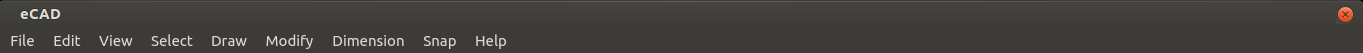
\includegraphics[width=0.9\textwidth]{images/menubar.png}
\caption{Menubar}
\end{figure}
\begin{enumerate}
\item \textbf{File Menu}: It consists of the following submenus.
\begin{itemize}
\item New: On clicking New menuitem we can create a new drawing. The shortcut key to it is Ctrl+N.
\item Open: This option will allow you to open a file which is already saved, so that one can edit it as per user requirement. The shortcut key is Ctrl+O.
\item Save: On clicking this one can save the new file if already not saved or save the existing modified file in xml format. The shortcut to it is Ctrl+S.
\item Save As: The Save As functionality allows to save the new file. The shortcut to it is Ctrl+Shift+S.
\item Import: Using this one can import the file from outside source. One can import jpg and png images in eCAD.
\item Export: Also sometimes the file needs to be exported in different formats. In eCAD one can export the file in the pdf, jpg and png formats.
\item Close: On clicking this the current drawing gets closed.
\item Print preview: Before printing user may want to view the file to print. This can be done by clicking this option or by pressing Ctrl+Shift+P. 
\item Print: To print the file click on it or press Ctrl+P.
\item Quit: To quit or close the software click on it or press Ctrl+Q.
\end{itemize}
\item \textbf{Edit Menu}: It contains the following submenus
\begin{itemize}
\item Cut: To cut the item click on it or press Ctrl+X.
\item Copy: To copy the item click on it or press Ctrl+C.
\item Paste: To paste the item click on it or press Ctrl+V.
\item Undo: To Undo click on it or press Ctrl+Z.
\item Redo: To Redo click on it or press Ctrl+Shift+Z.
\end{itemize}
\item \textbf{View menu}: It contains the following submenus
\begin{itemize}
\item Grid: On checking/unchecking it appears or disappears.
\item Zoom In: This option allows the view to zoom in.
\item Zoom out: On clicking it the view gets zoomed out.
\item Panning: One can scroll the drawing workspace using this feature.
\item Status Bar: This shows the current mouse position and also specifies the instructions to draw the entities.
\item Tool Bar: It futher have submenus for toolbar, scripting widgets and console mode.
\end{itemize}
\item \textbf{Select}: It contains the following submenus
\begin{itemize}
\item Select all: This will select all the entities
\item Deselect all: This will deselect all entites 
\item Select Window: This will select full window
\item Select entity: This will allow to select one entity
\item Deselect window: This will deselect window 
\item Invert Selection: This will invert the selection.
\end{itemize}
\item \textbf{Draw}: It contains the following submenus
\begin{itemize}
\item Points: It is used to draw points.
\item Line: It is used to draw Line.
\item Circle: It is used to draw Circle.
\item Ellipse: It is used to draw ellipse.
\item Arc: It is used to draw arc.
\item Text: It is used to add the text.
\item Image: It is used to add the image.
\end{itemize}
\item \textbf{Modify} : It contains the following submenus
\begin{itemize}
\item Delete selected: It will delete all the selected items.
\item Delete entity: It will delete the single entity. 
\end{itemize}
\item \textbf{Dimension}: It contains the following submenus
\begin{itemize}
\item Horizontal: It will allow to do the horizontal dimensioning.
\item Vertical: It allows to do vertical dimensioning.
\item Radial: It allows radial dimensioning too.
\item Diametric: It has an option for diametric dimensioning too.
\end{itemize}
\item \textbf{Snap}: It contains the following submenus
\begin{itemize}
\item Free: It will be free snap.
\item Grid: It will be for snap to grid. 
\item Center: It will be for snap to center
\item Middle Points: It will be for snap to mid points
\item End points: It will be for snap to end points
\end{itemize}
\item \textbf{Help}: It contains following submenus
\begin{itemize}
\item Manual: It will open the manual of the eCAD, that you are currently reading.
\item About: It will give brief description regarding license and developers of eCAD.
\end{itemize}
\end{enumerate}
\newpage
\subsection{Toolbar}
\begin{figure}[h!]
\centering

\includegraphics[width=0.9\textwidth]{images/toolbar.png}
\caption{Toolbar}
\end{figure}
Toolbar contains the shortcuts to various items in menubar. Like new, open, save, close, undo, redo etc. There are two toolbar standard toolbar and main toolbar.
\begin{enumerate}
\item \textbf{Main Toolbar}
\begin{figure}[h!]

\includegraphics[width=0.05\textwidth]{images/newDrawing.jpg} 
This creates a new drawing.
\end{figure}
\begin{figure}[h!]

\includegraphics[width=0.05\textwidth]{images/openDrawing.jpg} 
This opens a drawing.
\end{figure}
\begin{figure}[h!]

\includegraphics[width=0.05\textwidth]{images/saveDrawing.jpg} 
This saves a drawing.
\end{figure}
\begin{figure}[h!]

\includegraphics[width=0.05\textwidth]{images/cut.jpg} 
This cuts the selected entity.
\end{figure}
\begin{figure}[h!]

\includegraphics[width=0.05\textwidth]{images/copy.jpg} 
This copies the selected entity.
\end{figure}
\begin{figure}[h!]

\includegraphics[width=0.05\textwidth]{images/paste.jpg} 
This paste the entity at the position.
\end{figure}
\begin{figure}[h!]

\includegraphics[width=0.05\textwidth]{images/undo.jpg} 
This undo the previous action.
\end{figure}
\begin{figure}[h!]

\includegraphics[width=0.05\textwidth]{images/redo.jpg} 
This redo the previous action.
\end{figure}
\item \textbf{Standard ToolBar}
\begin{figure}[h!]

\includegraphics[width=0.05\textwidth]{images/point.jpg} 
This will create points
\end{figure}
\begin{figure}[h!]

\includegraphics[width=0.05\textwidth]{images/line.jpg} 
This will create line
\end{figure}
\begin{figure}[h!]

\includegraphics[width=0.05\textwidth]{images/circle.jpg} 
This will create circle
\end{figure}
\begin{figure}[h!]

\includegraphics[width=0.05\textwidth]{images/ellipse.jpg} 
This will create ellipse
\end{figure}
\begin{figure}[h!]

\includegraphics[width=0.05\textwidth]{images/arc.jpg} 
This will create arc
\end{figure}
\begin{figure}[h!]

\includegraphics[width=0.05\textwidth]{images/text.jpg} 
This will insert text using text editor interaction.
\end{figure}
\begin{figure}[h!]

\includegraphics[width=0.05\textwidth]{images/image.jpg} 
This will insert an image.
\end{figure}
\end{enumerate}
\vspace{30em}
\subsection{Working Space}
\begin{figure}[h!]
\centering
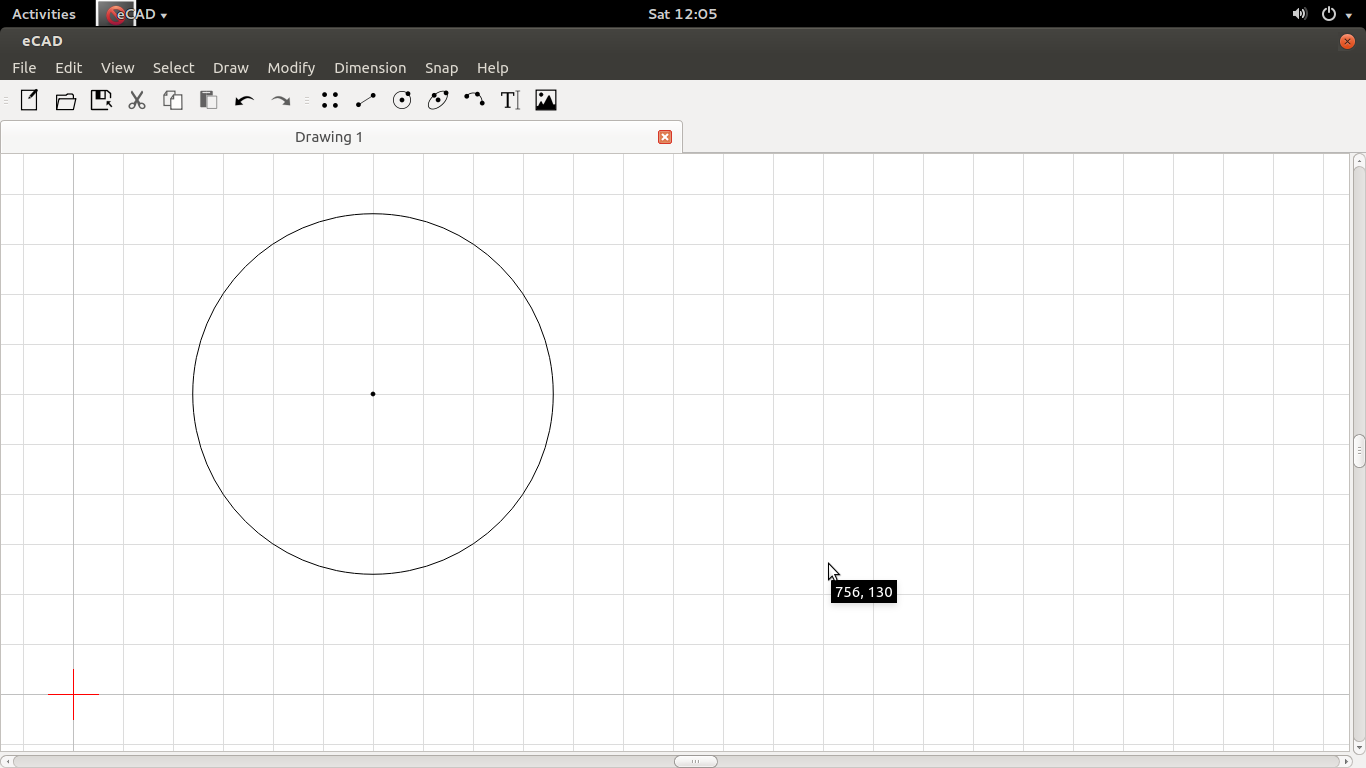
\includegraphics[width=0.9\textwidth]{images/drawingarea.png} 
\caption{Working Space}
\end{figure}
This is the working space where all the entities are drawn. One can increase or decrease the working area by closing or opening the widgets like scripting console and status bar. At present they are closed. This is the maximum area one will get to work. One can also make more than one drawing so that he/she can work easily. All depends upon user needs.
\subsection{Scripting Console}
\begin{figure}[h!]
\centering
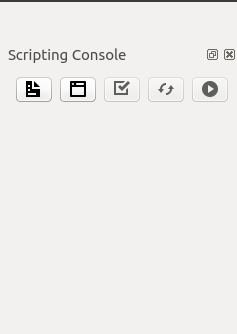
\includegraphics[width=0.4\textwidth]{images/scriptingconsole.png} 
\caption{Scripting console}
\end{figure}
In scripting console user can write the script/code to draw the drawing. So this feature is effective for technical users, who is excited and want to code. The code for each entity is very simple. There are different icons provided with the scripting console. Each have its different meaning.
\begin{figure}[h!]
\includegraphics[width=0.05\textwidth]{images/drawing.png} 
This will allow to create new script using javascript engine.
\begin{figure}[h!]

\includegraphics[width=0.05\textwidth]{images/browser.png} 
This will load an existing script.
\end{figure}
\begin{figure}[h!]

\includegraphics[width=0.05\textwidth]{images/task.png} 
This will save the script. The script is saved as \lq 1.js \rq.
\end{figure}
\begin{figure}[h!]

\includegraphics[width=0.05\textwidth]{images/loop-circular.png} 
This will clear the scripting console.
\end{figure}
\begin{figure}[h!]

\includegraphics[width=0.05\textwidth]{images/play-circular.png} 
This will execute the current script.
\end{figure}
\newpage
\subsection{Status Bar}
\begin{figure}[h!]
\centering

\includegraphics[width=0.9\textwidth]{images/statusbar.png} 
\caption{Status Bar}
\end{figure}
The status bar tells us about two things
\begin{itemize}
\item Current mouse position
\item What to do next while making an entity.
\end{itemize}